% \VignetteEngine{knitr::knitr}
\documentclass{bmcart}\usepackage[]{graphicx}\usepackage[]{color}
%% maxwidth is the original width if it is less than linewidth
%% otherwise use linewidth (to make sure the graphics do not exceed the margin)
\makeatletter
\def\maxwidth{ %
  \ifdim\Gin@nat@width>\linewidth
    \linewidth
  \else
    \Gin@nat@width
  \fi
}
\makeatother

\definecolor{fgcolor}{rgb}{0.345, 0.345, 0.345}
\newcommand{\hlnum}[1]{\textcolor[rgb]{0.686,0.059,0.569}{#1}}%
\newcommand{\hlstr}[1]{\textcolor[rgb]{0.192,0.494,0.8}{#1}}%
\newcommand{\hlcom}[1]{\textcolor[rgb]{0.678,0.584,0.686}{\textit{#1}}}%
\newcommand{\hlopt}[1]{\textcolor[rgb]{0,0,0}{#1}}%
\newcommand{\hlstd}[1]{\textcolor[rgb]{0.345,0.345,0.345}{#1}}%
\newcommand{\hlkwa}[1]{\textcolor[rgb]{0.161,0.373,0.58}{\textbf{#1}}}%
\newcommand{\hlkwb}[1]{\textcolor[rgb]{0.69,0.353,0.396}{#1}}%
\newcommand{\hlkwc}[1]{\textcolor[rgb]{0.333,0.667,0.333}{#1}}%
\newcommand{\hlkwd}[1]{\textcolor[rgb]{0.737,0.353,0.396}{\textbf{#1}}}%

\usepackage{framed}
\makeatletter
\newenvironment{kframe}{%
 \def\at@end@of@kframe{}%
 \ifinner\ifhmode%
  \def\at@end@of@kframe{\end{minipage}}%
  \begin{minipage}{\columnwidth}%
 \fi\fi%
 \def\FrameCommand##1{\hskip\@totalleftmargin \hskip-\fboxsep
 \colorbox{shadecolor}{##1}\hskip-\fboxsep
     % There is no \\@totalrightmargin, so:
     \hskip-\linewidth \hskip-\@totalleftmargin \hskip\columnwidth}%
 \MakeFramed {\advance\hsize-\width
   \@totalleftmargin\z@ \linewidth\hsize
   \@setminipage}}%
 {\par\unskip\endMakeFramed%
 \at@end@of@kframe}
\makeatother

\definecolor{shadecolor}{rgb}{.97, .97, .97}
\definecolor{messagecolor}{rgb}{0, 0, 0}
\definecolor{warningcolor}{rgb}{1, 0, 1}
\definecolor{errorcolor}{rgb}{1, 0, 0}
\newenvironment{knitrout}{}{} % an empty environment to be redefined in TeX

\usepackage{alltt}

\usepackage{xcolor}
\usepackage{url}
\usepackage{amsmath}
\usepackage{amsthm}
\usepackage{amssymb}
\usepackage{graphicx}
\usepackage{tikz}
\usetikzlibrary{shapes,arrows}
\usepackage{float}
\usepackage{verbatim}
\usepackage{hyperref}
\hypersetup{
     colorlinks   = true,
     citecolor    = black
}
\hypersetup{linkcolor=black}
% \hypersetup{linkcolor=black}
% \hypersetup{linkcolor=black}


% \usepackage{authblk}
\usepackage[utf8]{inputenc} %unicode support
\IfFileExists{upquote.sty}{\usepackage{upquote}}{}
\begin{document}

%\maketitle


\begin{frontmatter}

\begin{fmbox}
\dochead{Draft}

\title{High Resolution Identification of Protein-DNA Binding
  Events and Quality Control for ChIP-exo data}

\author[
   addressref={aff6},                   % id's of addresses, e.g. {aff1,aff2}
   email={chungd@musc.edu}   % email address
]{\inits{DC}\fnm{Dongjun} \snm{Chung}}
\author[
   addressref={aff1},
   email={welch@stat.wisc.edu}
]{\inits{RW}\fnm{Rene} \snm{Welch}}
\author[
   addressref={aff3},
   email={ong@cs.wisc.edu}
]{\inits{IO}\fnm{Irene} \snm{Ong}}
\author[
   addressref={aff3,aff4},
   email={jagrass@wisc.edu}
]{\inits{JG}\fnm{Jeffrey} \snm{Grass}}
\author[
   addressref={aff3,aff4,aff5},
   email={landick@bact.wisc.edu}
]{\inits{RL}\fnm{Robert} \snm{Landick}}
\author[
   addressref={aff1,aff2},
   corref={aff1},
   email={keles@stat.wisc.edu}
]{\inits{SK}\fnm{S\"und\"uz} \snm{Kele\c{s}}}



\address[id=aff1]{%                           % unique id
  \orgname{Department of Statistics, University of Wisconsin Madison}, % university, etc
  \street{1300 University Avenue},                     %
  %\postcode{}                                % post or zip code
  \city{Madison},                              % city
  \cny{WI}                                    % country
}

\address[id=aff2]{%
  \orgname{Department of Biostatistics and Medical Informatics, University of Wisconsin Madison},
  \street{600 Highland Avenue},
%  \postcode{24105}
  \city{Madison},
  \cny{WI}
}
\address[id=aff3]{
  \orgname{Great Lakes Bioenergy Research Center, University of Wisconsin Madison},
  \street{1552 University Avenue},
  \city{Madison},
  \cny{WI}
}
\address[id=aff4]{
  \orgname{Department of Biochemistry, University of Wisconsin Madison},
  \street{433 Babcock Drive},
  \city{Madison},
  \cny{WI}
}
\address[id=aff5]{
  \orgname{Department of Bacteriology, University of Wisconsin Madison},
  \street{1550 Linden Drive},
  \city{Madison},
  \cny{WI}
}
\address[id=aff6]{
  \orgname{Department of Public Health Sciences, Medical University of South Carolina},
  \street{135 Cannon Street},
  \city{Charleston},
  \cny{SC}
}


% \begin{artnotes}
% %\note{Sample of title note}     % note to the article
% \note[id=n1]{Equal contributor} % note, connected to author
% \end{artnotes}


\end{fmbox}

\begin{abstractbox}

  \begin{abstract}

    Recently, ChIP-exo has been developed to investigate protein-DNA
    interaction in higher resolution compared to popularly used
    ChIP-Seq. Although ChIP-exo has drawn much attention and is
    considered as powerful assay, currently, no systematic studies
    have yet been conducted to determine optimal strategies for
    experimental design and analysis of ChIP-exo. In order to address
    these questions, we evaluated diverse aspects of ChIP-exo and
    found the following characteristics of ChIP-exo data. First, the
    background of ChIP-exo data is quite different from that of
    ChIP-Seq data. However, sequence biases inherently present in
    ChIP-Seq data still exist in ChIP-exo data. Second, in ChIP-exo
    data, reads are located around binding sites much more tightly and
    hence, it has potential for high resolution identification of
    protein-DNA interaction sites, and also the space to allocate the
    reads is greatly reduced. Third, although often assumed in the
    ChIP-exo data analysis methods, the ``peak pair'' assumption does
    not hold well in real ChIP-exo data. Fourth, spatial resolution of
    ChIP-exo is comparable to that of PET ChIP-Seq and both of them
    are significantly better than resolution of SET ChIP-Seq. Finally,
    for given fixed sequencing depth, ChIP-exo provides higher
    sensitivity, specificity and spatial resolution than PET
    ChIP-Seq.

    In this article we provide a quality control pipeline which
    visually assess ChIP-exo biases and calculates a signal-to-noise
    measure. Also, we updated dPeak \cite{dpeak}, which makes a
    striking balance in sensitivity, specificity and spatial
    resolution for ChIP-exo data analysis.

\end{abstract}

\begin{keyword}
  \kwd{ChIP-exo}
  \kwd{QC}
  \kwd{TFBS}
  \kwd{BS identification on High-Res}
\end{keyword}

\end{abstractbox}

\end{frontmatter}

\newpage

\listoffigures

\newpage

\section{Background}
\label{sec:intro}

ChIP-exo (Chromatin Immunopecipitation followed by exonuclease
digestion and next generation sequencing) Rhee and Pugh (\cite{exo1})
is the state-of-the-art experiment developed to attain single
base-pair resolution of protein binding site identification and it is
considered as a powerful alternative to popularly used ChIP-Seq
(Chromatin Immunoprecipitation coupled with next generation sequencing
) assay. ChIP-exo experiments first capture millions of DNA fragments
(150 - 250 bp in length) that the protein under study interacts with
using random fragmentation of DNA and a protein-specific
antibody. Then, exonuclease is introduced to trim 5' end of each DNA
fragment to a fixed distance from the bound protein. As a result,
boundaries around the protein of interest constructed with 5' ends of
fragments are located much closed to bound protein compared to
ChIP-Seq. This step is unique to ChIP-exo and could potentially
provide significantly higher spatial resolution compared to
ChIP-Seq. Finally, high throughput sequencing of a small region (25 to
100 bp) at 5' end of each fragment generates millions of reads or
tags.

While the number of produced ChIP-exo data keeps increasing,
characteristics of ChIP-exo data and optimal strategies for
experimental design and analysis of ChIP-exo data are not fully
investigated yet, including issues of sequence biases inherent to
ChIP-exo data, choice of optimal statistical methods, and
determination of optimal sequencing depth. However, currently the
number of available ChIP-exo data is still limited and their
sequencing depths are still insufficient for such investigation. To
address this limitation we gathered ChIP-exo data from diverse
organisms: CTCF factor in human \cite{exo1}; ER factor in human and
FoxA1 factor in mouse \cite{exoillumina}; and generated $\sigma^{70}$
factor in Escherichia coli (E. Coli) under aerobic ($ + O_2$)
condition, and treated by rifampicin by 0 and 20 minutes.

DNA libraries generated by the ChIP-exo protocol seem to be less
complex than the libraries generated by ChIP-Seq
\cite{exo_review}. Hence, most of current QC guidelines
\cite{encode_qc} may not be applicable on ChIP-exo, additionally to
our knowledge there are not established quality control pipelines for
ChIP-exo. To address this challenge, we suggest a collection of
quality control visualizations to understand which biases are present
in ChIP-exo data. Previous ChIP-exo analysis used ChIP-Seq samples to
compare the resolution between experiments (\cite{exo1}, \cite{exo2},
\cite{exoillumina}); in \cite{carroll.qc}, Carroll et. al. studied the
use of the Strand-Cross Correlation (SCC) \cite{strandcc} and showed
that by filtering blacklisted regions the estimation of the SCC is
improved. However, this method requires to know blacklisted regions in
advance which may not be available, additionally using SCC may not be
useful since the peaks that are attained at the read and fragment
length are confused in a typical ChIP-exo SCC curve.  In our pipeline
we propose two out-the-shelf analysis: An enrichment plot and the
local normalized SCC cofficient.

In order to archive the potential benefits of ChIP-exo on protein
binding site identification, it is critical to understand which are
the important characteristics of ChIP-exo data and to use algorithms
that could fully utilize information available in ChIP-exo data. Rhee
and Pugh \cite{exo1} discussed that reads in the forward and reverse
strand might construct peak pairs around bound protein, of which
heights were implicitly assumed to be symmetric. Hence, they used the
``peak pair method'' that predicts the midpoint of two modes of peak
pairs as potential binding site. Mace \cite{mace}, CexoR \cite{cexor}
and peakzilla \cite{peakzilla}, recently developed ChIP-exo data
analysis methods, are also based on this peak pair
assumption. However, appropriateness of such assumption was not fully
evaluated in the literature yet.  Furthermore, it is still unknown
which factors could affect protein binding site identification using
ChIP-exo data. In order to address this problem, we investigated
various aspects of ChIP-exo data by contrasting them with their
respective ChIP-Seq experiments.

Currently, research on statistical methods for ChIP-exo data is still
in its very early stage. Although many methods have been proposed to
identify protein binding sites from ChIP-Seq data (reviewed in
\cite{evaluation} and \cite{computation}), such as MACS \cite{macs},
CisGenome \cite{cisgenome} and MOSAiCS \cite{mosaics}, these
approaches reveal protein binding sites in lower resolution, i.e., at
an interval of hundreds to thousands of base pairs. Furthermore, they
report only one ``mode'' or ``predicted binding location'' per
peak. Hence, these methods are not appropriate to evaluate the
potential of ChIP-exo data for high resolution identification of
protein binding sites. More recently, deconvolution algorithms such as
Deconvolution \cite{csdeconv}, GEM \cite{gem} (an improved version of
\cite{gps}) and PICS \cite{pics} have been proposed to identify
binding sites in higher resolution using ChIP-Seq data. However, most
of them are still not tailored for ChIP-exo and PET and SET ChIP-Seq
data in a unified framework and as a result, currently available
methods are not appropriate for fair comparison between ChIP-exo and
ChIP-Seq. To address these limitations, we developed an improved of
dPeak \cite{dpeak}, a high resolution binding site identification
(deconvolution) algorithm that we previously developed for PET and SET
ChIP-Seq data, so that it can also handle ChIP-exo data. The dPeak
algorithm implements a probabilistic model that accurately describes
the ChIP-exo and ChIP-Seq data generation process.

In this paper, we demonstrate that the ``peak pair'' assumption of
Rhee and Pugh \cite{exo1} does not hold well in real ChIP-exo
data. Furthermore, we found that when we analyze ChIP-exo data from
eukaryotic genomes, it is important to consider sequence biases
inherent to ChIP-exo data, such as mappability and GC content in order
to improve sensitivity and specificity of binding site
identification. We evaluated several method to identify binding events
and dPeak outperforms or performs competitively respecto to GEM and
MACE when analyzing ChIP-exo data. More importantly, when comparable
number of reads is used for both ChIP-exo and ChIP-Seq, dPeak coupled
with ChIP-exo data provides resolution comparable to PET ChIP-Seq and
both significantly improve the resolution of protein binding site
identification compared to SET-based analysis with any of the
available methods.

\newpage

\section{Results and discussion}
\label{sec:results}

\subsection{Deeply sequenced E.Coli $\sigma^{70}$ ChIP-exo and ChIP-Seq data}
\label{sec:ourdata}

$\sigma^{70}$ factor is a transcription initiation factor of
housekeeping genesin E. coli. In E. coli genomes, many promoters
contain multiple transcription start sites (TSS) and these TSS are
often closely space (10 ~ 150 bp). These closely spaced binding sites
are considered to be multiple ``switches'' that differentially
regulate gene expression under diverse growth conditions
\cite{regdb_old}, \cite{regulondb}. Therefore, investigation of
ChIP-exo's potential for identification and differentiation of closely
spaced binding sites are invaluable for elucidating the
transcriptional networks of prokaryotic genomes.

\subsection{Current guidelines and quality metrics}
\label{sec:qcnow}

We calculated the most commonly used quality indicators for ChIP-Seq
data, which are listed in table \ref{tab:qcbase}. The PBC and NSC were
calculated as defined in \cite{encode_qc} and the SSD was calculated
as defined in \cite{htseq}. Additionally, we calculated the FSR to
compare the number of fragments in each strand. A few conclusions that
we may get by observing the PBC in table \ref{tab:qcbase} are all the
samples have a quite low library complexity, hence it would be
suggested to repeat the experiment.

\begin{table}[h]
  \centering
\begin{tabular}{l|r|r|r|r|r|r}
\hline\hline
Condition & Rep. & Nr. reads & PBC & SSD & FSR & NSC  \\
\hline\hline
Rif-0min & 1 & 960,256 & 0.2823 & 0.0361 & 0.4998 & 10.29 \\
\hline
Rif-0min & 2 & 2,247,295 & 0.2656 & 0.1091 & 0.5047 &  25.08  \\
\hline
Rif-20min & 1 & 1,940,387 & 0.2698 & 0.0820 & 0.5054 & 17.69  \\
\hline
Rif-20min & 2 & 4,229,574 & 0.2153 & 0.1647 & 0.5071 &  14.11 \\
\hline
\end{tabular}  
\caption{Usual quality control indicators applied to our
  $\sigma^{70}$ samples. PBC stands PCR-bottleneck coefficient, SSD
  for standardized standard deviation, FSR for forward strand ratio,
  NSC for normalized strand cross-correlation coefficient. We
  omitted the RSC (relative strand cross-correlation since ChIP-exo
  experiments don't usually have an accompanying input file) 
  [note: I need to change the table, due the alignment issue]}

  \label{tab:qcbase}
\end{table}

\begin{figure}[h!]
  \centering
  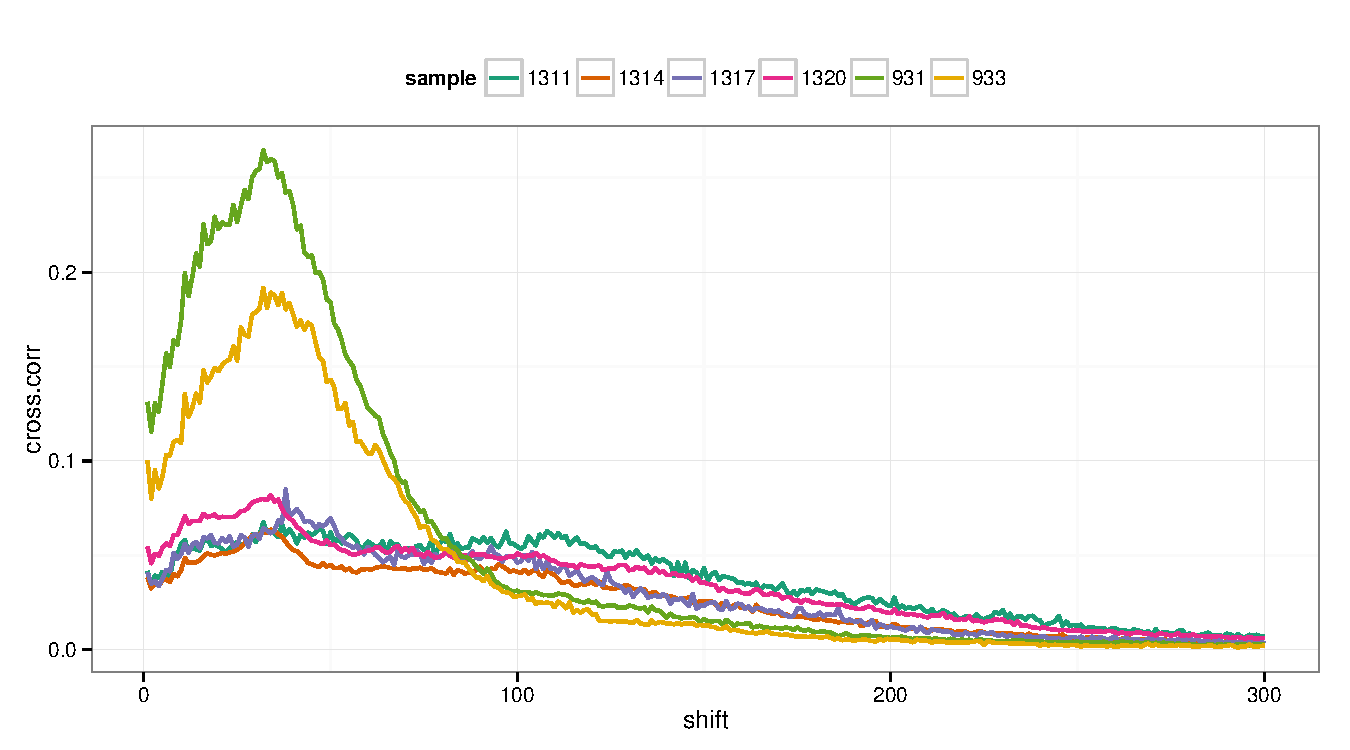
\includegraphics[width = .8\textwidth]{../figs/for_paper/EColi_strand_cross_corr.pdf}
  \caption{Strand cross-correlation curves for $\sigma^{70}$
    samples. The ``phantom peak'' and the summit that corresponds to
    the read and fragment length respectively are confounded, due to
    the exonuclease enzyme digestion.}
  \label{figsup:scc}
\end{figure}

It is of special importance to notice that the vlaues of PBC or are
quite low, hence these experiment would be repited if there were
considered as ChIP-Seq experiments. On the other hand, in a good
ChIP-Seq experiment the strand cross-correlation is maximized at the
fragment length and there is also a ``phantom peak'' at the sample's
read length (\cite{encode_qc} and \cite{strandcc}).  However, in
ChIP-exo's case this two peaks are confounded. Hence an enrichment
measure based in the strand cross-correlation such as NSC or RSC is
harder to interpret. In figure \ref{figsup:scc} we plotted the SCC
curves for $\sigma^{70}$ ChIP-exo experiments used to calculate the
NSC and RSC values in table \ref{tab:qcbase}. According to ENCODE's
quality metrics, NSC values close to one corresponds to low enrichment
samples or bad quality datasets, hence in our case the last four
samples would be considered to have higher quality than they actually
have. On the other hand, all PBC values are considerably low and
correspond to samples with severe bottlenecking issues, in particular
we are going to show that for the first two samples we are obtaining a
smaller resolution and identifying a comparable number of targets as
in ChIP-Seq PET experiments.

\subsection{ChIP-exo Quality Control pipeline}
\label{sec:QC}

Figure \ref{fig:qcdiagram} shows a flowchart for the ChIPexoQC
pipeline. Which basically partitions the genome by keeping the
non-digested ChIP-exo regions. Then, for each region it calculates a
series of statistics. Finally, it creates several visualizations
designed to assess the quality levels of a ChIP-exo sample.

\begin{figure}[h!]
  \centering
  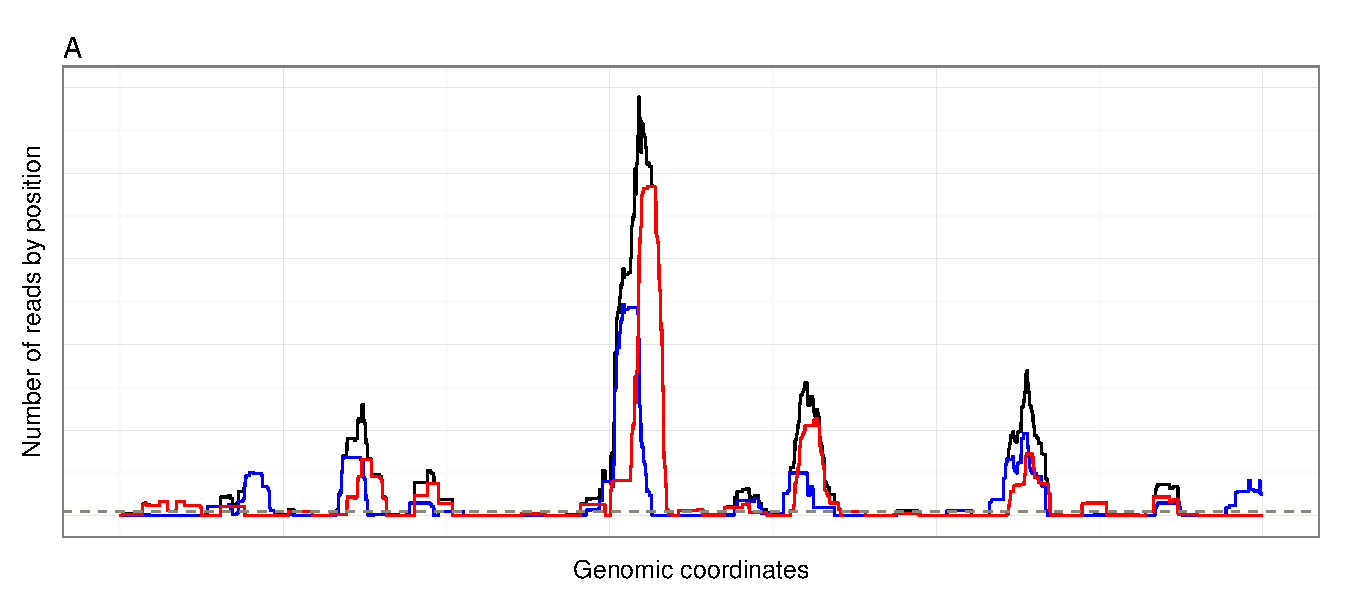
\includegraphics[width = .9\textwidth]{../figs/for_paper/coverage_diagram.pdf}
  \caption{Diagram of the ChIP-exo Quality control pipeline [this is a
    place-holder]. The genome is partitioned into several regions by
    removing the empty segments and for each regions we calculate a
    collection of QC indicators.}
  \label{fig:qcdiagram}
\end{figure}

\subsubsection{Enrichment and library complexity in ChIP-exo data}
\label{sec:enri}

In ChIP-exo experiments, the background is often digested by the
exonuclease enzyme, therefore to determine the sample's quality is
necessary to address the balance between the enrichment and library
complexity. To diagnose this, we considered the Average Read Coverage
(ARC) and the Unique Read Coverage Rate (URCR) which are defined as:

\begin{align}
  \mbox{ARC} &= \frac{\text{Nr. of reads in the region}}{\text{Width of the region}} \nonumber \\
  \mbox{URCR} &= \frac{\text{Nr. of reads mapped to only one position
      in the region}}{\text{Nr. of reads in the region}} \nonumber
\end{align}

Using the mouse-FoxA1 experiment from \cite{exoillumina} and the
relationship between this two quantities, library complexity and
sample enrichment was explored. Figure \ref{fig:enrich}A shows hexbin
plots illustrating the interaction between these two
quantities. Notice how there are two strong arms in each panel: The
first one corresponds to regions with low $\mbox{ARC}$ values and
varying $\mbox{URCR}$ values across the $(0,1]$ interval, while the
second one shows a decreasing trend in $\mbox{URCR}$ as $\mbox{ARC}$
increases. When an experiment shows a higher degree of enrichment,
then the separation of this two arms is more noticeable, since the
second arm corresponds to possibly enriched regions
(\ref{fig:enrich2}A and \ref{fig:enrich2}B).



Figure \ref{fig:enrich}B shows box plots of the $\mbox{local-NSC}$ on
regions of the three replicates, stratified by the number of reads
mapped exactly to one position for all $\sigma^{70}$ ChIP-exo
experiments; The high stratum is defined by regions consisting of more
than 100 unique positions, the medium stratum for regions
where the number of unique position is on the
(50,100) range and the low stratum in the
(20,50) range. For each stratum and biological
replicate, we sampled 400 regions whenever possible (in the
opposite case, all the regions in the category were considered) and
calculated the $\mbox{local-NSC}$ for those regions. For all three
replicates, it is shown an increasing trend as the number of unique
position increases, which means that the $\mbox{local-NSC}$ is an
effective indicator of library complexity. Figure \ref{fig:enrich}C
shows the $\mbox{local-NSC}$ coefficient calculated for the same set
of regions, stratified by the number of unique positions in the
regions of ERR336942 using the same criteria as before. In the high
panel it is shown that the ERR336942 sample performs slightly better
than ERR336956 and both outperform ERR336935, this agrees with
\ref{fig:enrich}A, where only in the left-most panel doesn't seem to
be a separation between the low $\mbox{ARC}$ arm and the other.

\emph{Comment: I think I need to change the name of the FoxA1 samples
  to Rep1 to Rep3, but I wasn't sure about this. Therefore I used the
  name of the bam files}

\begin{figure}[h!]
  \centering
  \includegraphics[width = .8\textwidth]{../figs/Carroll_mice_for_paper/FoxA1_enrichment.pdf}
  \includegraphics[width = .8\textwidth,page =3]{../figs/Carroll_mice_for_paper/Local_SCC_indicator_by_strata.pdf}
  \includegraphics[width = .8\textwidth,page =4]{../figs/Carroll_mice_for_paper/Local_SCC_indicator_by_strata_sameRegion.pdf}
  \caption{Using the mouse-FoxA1 experiment from \cite{exoillumina}:
    A) Hexbin plots of $\mbox{ARC}$ against $\mbox{URCR}$, in general
    we can see a slight separation into two strong arms, one
    corresponds to low $\mbox{ARC}$ and varying $\mbox{URCR}$, and for
    the other $\mbox{URCR}$ decreases as $\mbox{ARC}$ increases B)
    Boxplots of the $\mbox{local-NSC}$ stratified by nr. of reads
    mapped to only one position in the regions for the ChIP-exo
    experiments divided by condition and biological replicate and C)
    Boxplots of the a set of ERR336942 regions, stratified as in (B)
    with the $\mbox{local-NSC}$ calculated with the different
    biological replicates.}
  \label{fig:enrich}
\end{figure}


\subsubsection{Strand imbalance in ChIP-exo data}
\label{sec:strand_imbalance}

The strand imbalance assessment is based in the observation that the
enriched regions usually have a higher concentration of fragments,
therefore we examined the FSR (defined as the ratio of the number of
forward stranded reads divided by the total number of reads in a given
region) as the region with lower depth are being filtered out. This
indicator is of particular importance, since several methods rely on
the ``peak-pair'' assumption. In table \ref{tab:qcbase}, we calculated
the FSR and noticed that for all the samples, it's value is close to
0.5, which means that there are roughly the same amount of reads in
both strands. However, figure \ref{fig:comp}B shows that this value is
not representative of the sample locally, therefore the assumption
doesn't hold in practice.



In order to assess the strand imbalance we created the following
visualization presented in figure \ref{fig:strand}. A) shows the FSR's
behavior as lower depth regions are being filtered out, while B) shows
which percentage of the regions are composed by fragments of both
strands or only one (forward or backward). As the number of reads per
region's lower bound increases, the quantiles tend to approach the
median. To evaluate this statement, for each replicate of the FoxA1
dataset, we divided the regions formed by at least 100
fragments into into the ones that overlap with any of the sample's
peaks. The p.value for ERR36935 is 0.1039, for ERR336942 is
0.0064 and for ERR336956 is 0.0871. This shows
that only the middle sample from figure \ref{fig:strand} is the least
imbalance sample from the the three, while the other two still show a
higher imbalance at the 100 level.

\begin{figure}[h!]
  \centering  
  \includegraphics[width = .8\textwidth,page = 3]{../figs/Carroll_mice_for_paper/Strand_imbalance.pdf} 
  \caption{Strand imbalance QC plots for the same data as in figure
    \ref{fig:enrich}. A) FSR distribution quantiles as the lower depth
    regions are being filtered out, all quantiles approach to the
    median as the lower bound increases. B) Stacked histogram with the
    proportion of regions that are formed by two strands or only one,
    in a good sample the single-stranded regions are going to be
    filtered out quickly as in the middle row.}
  \label{fig:strand}
\end{figure}



\subsection{Comparison with ChIP-Seq data}
\label{sec:comp}



We first compared various factors that could affect binding site
identification between ChIP-exo and ChIP-Seq data. In order to compare
distribution of signal and background between ChIP-exo and ChIP-Seq
data, we calculated ChIP tag counts across the genome by counting the
number of reads mapping to each of 150 non-overlapping
window after extending reads by 150 to their 3' end
directions. ChIP tag counts in ChIP-exo data were linearly related to
ChIP tag counts in ChIP-Seq data for the regions with high ChIP tag
counts (Figure \ref{fig:comp}A). This implies that signals for
potential binding sites are well reproducible between ChIP-exo and
ChIP-Seq data. On the other hand, there was clear difference in the
background distribution between them. In ChIP-Seq data reads were
almost uniformly distributed over background (non-binding) regions and
the ChIP tag counts in there regions were significantly larger than
zero. In contrast, in ChIP-exo data, there was larger variation in
ChIP tag counts among background regions and ChIP tag counts were much
lower in these regions compared to ChIP-Seq data. There were also
large proportion of regions without any read in ChIP-exo data. These
results indicate that background distribution of ChIP-exo data is less
homogeneous than that of ChIP-Seq data.

We next evaluated the ``peak pair'' assumption from Rhee and Pugh
\cite{exo1}, MACE \cite{mace}, CexoR, \cite{cexor} and peakzilla
\cite{peakzilla}, i.e. a peak of reads in the forward strand is
usually paired with a peak of reads in the reverse strand that is
located in the other site of the binding site. In order to evaluate
this assumption, we reviewed the proportion of reads in the forward
strand in candidate regions (i.e. regions with at least one binding
site) in $\sigma^{70}$ ChIP-exo data. We found that strands of reads
were much less balanced in ChIP-exo data than in ChIP-Seq data in
these regions with potential binding sites (Fig. \ref{fig:comp}B) and
this indicates that the peak pair assumption might not hold in real
ChIP-exo data.

%  We obtained esentially the same conclusion from the
% ChIP-exo data for CTCF factor from human sample Rhee and Pugh
% (\cite{exo1}) as well. 

\begin{figure}[h]
  \centering
  \includegraphics[width = .46\textwidth,page = 3 ]{../figs/for_paper/ChIPseqPET_ChIPexo_tagCount_comparison.pdf}
  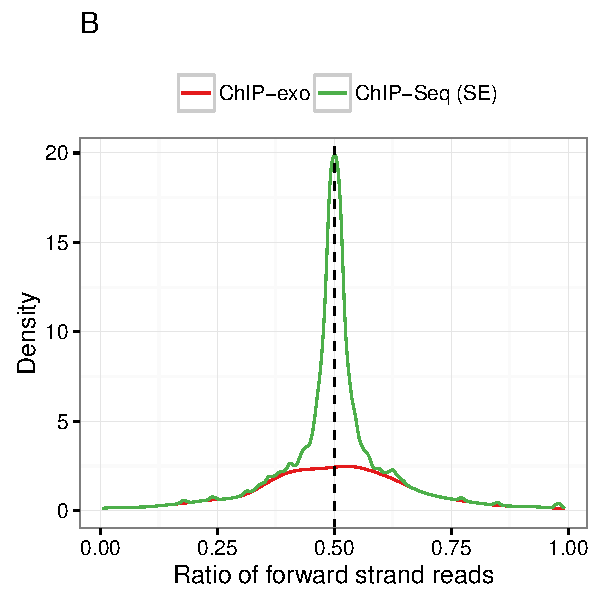
\includegraphics[width = .46\textwidth]{../figs/for_paper/forward_strand_ratio_comp_old.pdf}
  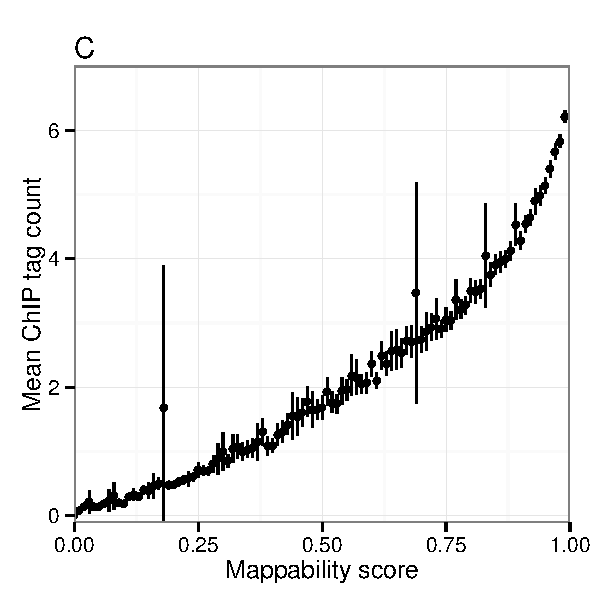
\includegraphics[width = .46\textwidth,page = 1]{../figs/for_paper/eukaryotic_bias_CTCF.pdf}
  \includegraphics[width = .46\textwidth,page = 2]{../figs/for_paper/eukaryotic_bias_CTCF.pdf}
  \caption{ A) ChIP signal in ChIP-exo was linearly related to that in
    PET ChIP-Seq data in the region with high ChIP tag counts. In
    contrast, there were clear differences in their background
    distribution, where several ChIP-exo background regions were
    empty. B) In ChIP-exo data, strands of reads were significantly
    less balanced in the regions with potential binding sites compared
    to SET ChIP-Seq data. C) ChIP tag counts increase linearly as
    mappability scores increases. D) ChIP tag counts increase linearly
    as GC content score increases when GC content is less than 0.6 and
    then ChIP tag counts decrease as GC content increases. }
  \label{fig:comp}
\end{figure}

\subsubsection{ChIP-exo data from eukaryotic genome shows clear sequence biases}
\label{sec:eukaryotic}

We evaluated ChIP-exo data for CTCF factor from human genome
\cite{exo1} to investigate issues specific to eukaryotic genomes for
binding sites identification. Figures \ref{fig:comp}C and
\ref{fig:comp}D display the bin-level average read counts against
mappability and GC content. Each data point is obtained by averaging
the read counts across bins with the same mappability of GC
content. These results indicate that binding site identification in
ChIP-exo sample might also benefit from the use of methods that take
into account of apparent sequence biases such as mappability and GC
content.


\subsubsection{Comparison with ChIP-Seq data using dPeak}
\label{sec:dpeak_analysis}



Figure \ref{fig:reso_all} shows different comparisons among ChIP-exo,
PET ChIP-Seq and SET ChIP-Seq. A RegulonDB annotation was considered
identified if the distance between it and dPeak binding site estimate
was at most of 20 bp. That way, the sensitivity is defined as
the proportion of RegulonDB annotations identified in a peak. In
figure \ref{fig:reso_all}A can be seen that the sensitivity of all
protocols increases as the average distance between binding sites
does. Despite that when the binding events in a peak are closer to
each other, both ChIP-exo and PET ChIP-Seq are comparable, as the
distance increases ChIP-exo identifies a higher proportion of the
RegulonDB annotations; additionally SET ChIP-Seq is significantly less
sensible than both ChIP-exo and PET ChIP-Seq. In figure
\ref{fig:reso_all}B the distance between a RegulonDB annotation to its
closest prediction is compared for ChIP-exo, PET and SET ChIP-Seq;
while the first two are comparable, both outperform SET ChIP-Seq.

In figures \ref{fig:reso_all}C and \ref{fig:reso_all}D, we observe the
behavior of dPeak's estimated parameters for single end data (both
ChIP-exo and ChIP-Seq). The $\delta$ parameter measures the distance
from the 5' end of the fragment to its respective binding event and
the $\sigma$ parameter indicates the fragments distribution
variability around their respective binding sites (more information in
\cite{dpeak}). For both parameters, it can be seen that the ChIP-exo
estimates are smaller than the SET ChIP-Seq estimates in average,
which agrees with the fact that the sample reads are allocated more
tightly around the binding events in ChIP-exo data. Hence we can
conclude that the peaks shape is quite different between ChIP-exo and
SET ChIP-Seq.


\begin{figure}[h!]
  \centering
  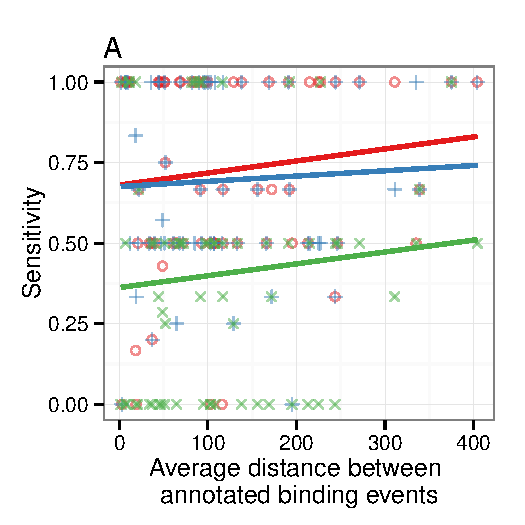
\includegraphics[width = .46\textwidth]{../figs/for_paper/sensitivity_exo_olda_data.pdf}
  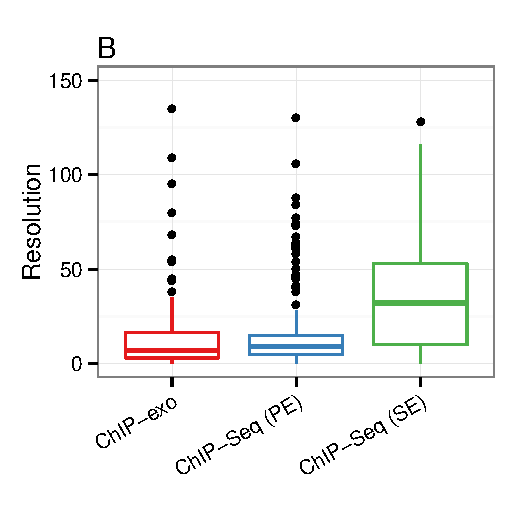
\includegraphics[width = .46\textwidth]{../figs/for_paper/resolution_by_dataset_old_data.pdf}
   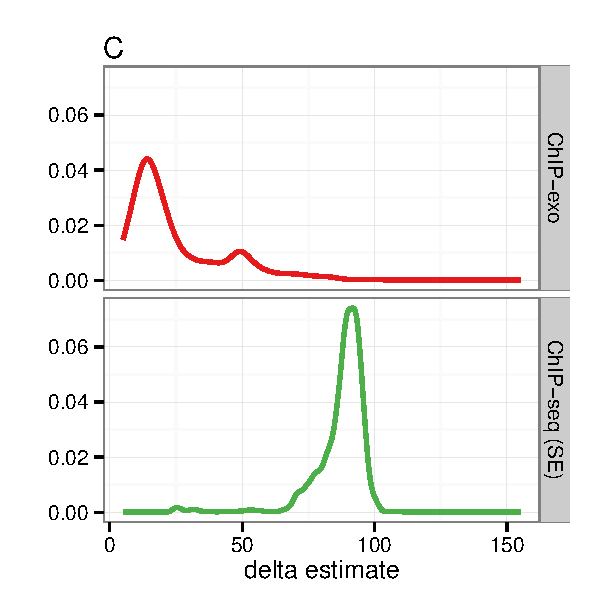
\includegraphics[width = .46\textwidth,page = 1]{../figs/for_paper/sigma_delta_old_densities.pdf}
   \includegraphics[width = .46\textwidth,page = 2]{../figs/for_paper/sigma_delta_old_densities.pdf} 

   \caption{Comparison of (A) sensitivity and (B) resolution between
     ChIP-exo and ChIP-Seq data. Sensitivity is defined as the
     proportion of RegulonDB annotations identified using each
     data. Resolution is defined as the distance between RegulonDB
     annotation and its closest prediction. $\quad$ C) $\delta$ parameter in
     dPeak measures average distance of the reads to their respective
     binding site. In ChIP-exo data, reads were located much closer to
     the binding site than in SET ChIP-Seq. D) $\sigma$ parameter
     measure the dispersion of reads around each binding site. In
     ChIP-exo data, reads showed less variation around the their
     respective binding sites compared to SET ChIP-Seq.}
  \label{fig:reso_all}
\end{figure}

\subsection{Recommendations for the design of ChIP-exo experiments}
\label{sec:reco}



We sampled a fixed amount of fragments for each of the ChIP-exo, PET
ChIP-Seq and SET ChIP-Seq datasets of the $\sigma^{70}$ sample in
aerobic conditions. For each sampled dataset we applied our
lower-to-higher resolution pipeline by calling peaks with MOSAiCS
\cite{mosaics} and then deconvolving the binding events by using dPeak
\cite{dpeak}. For the ChIP-exo datasets we called peaks by using
GC-content and mappability with MOSAiCS, and for the ChIP-Seq datasets
we used their respective Input samples.

\begin{figure}[h!]
  \centering
%  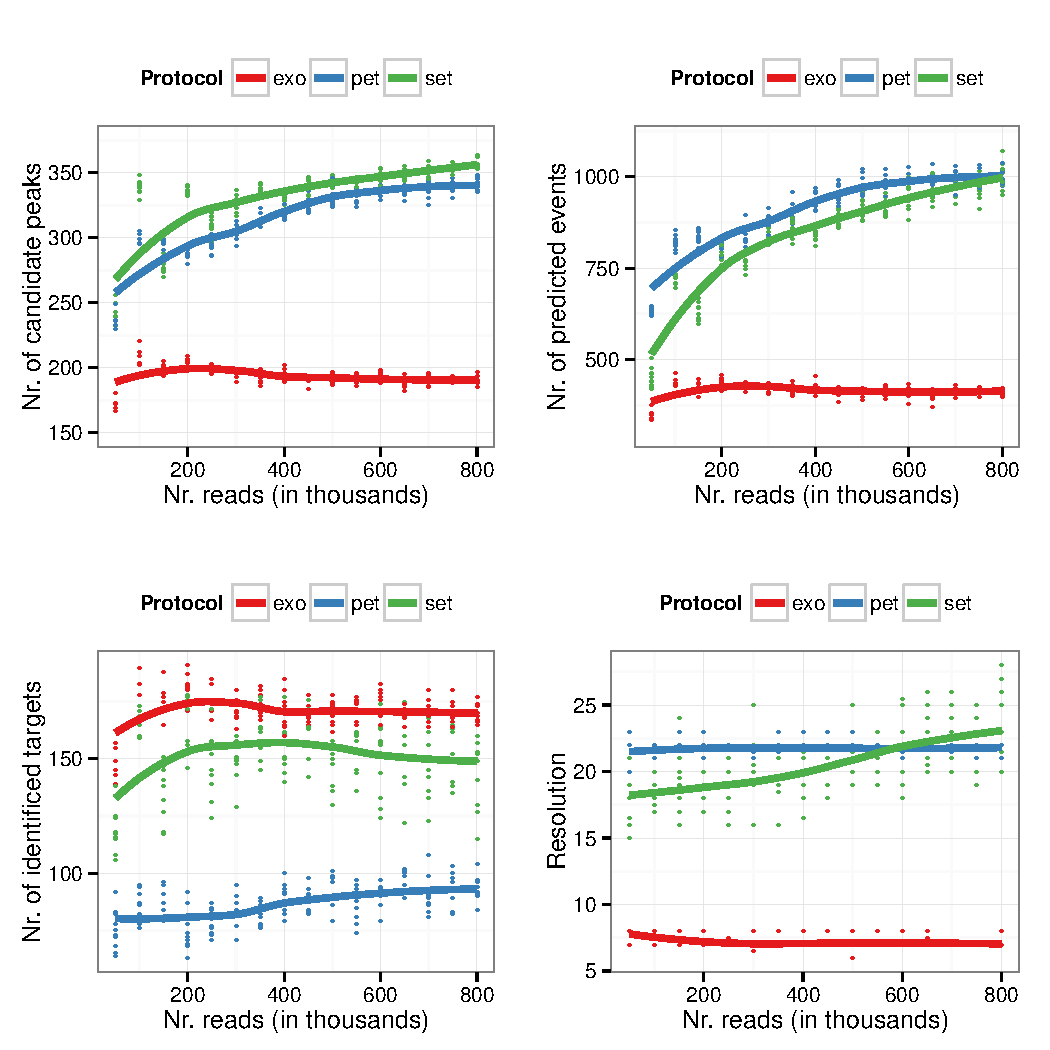
\includegraphics[width = .8\textwidth]{../figs/for_paper/Sig70_aerobic_saturation.pdf}
  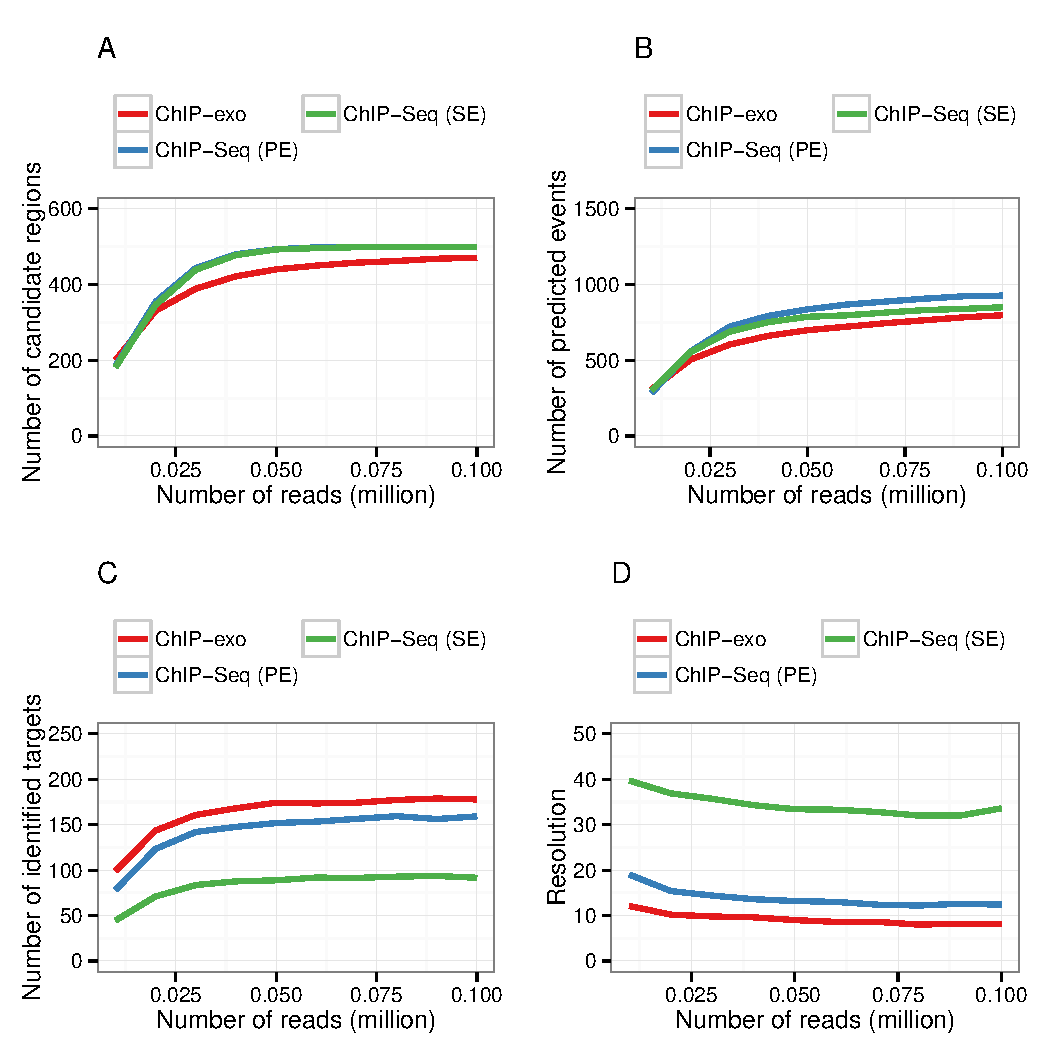
\includegraphics[width = .8\textwidth]{../figs/for_paper/saturation_analysis_old.pdf}
  \caption{Comparison of the number of candidate regions (A),
    predicted events (B), identified targets (C) and resolution (D)
    among ChIP-exo, PET ChIP-Seq and SET ChIP-Seq. RegulonDB
    annotations are considered as a gold standard. A gold standard was
    considered identified if a BS was estimated inside a 15
    bp window around it}
  \label{fig:design}
\end{figure}

Figure \ref{fig:design} shows the behavior of each data type when
their depth is fixed. It is remarkable that even when the number of
candidate peaks or the number of predicted events is lower for
ChIP-exo, it outperforms both PET and SET ChIP-Seq in the number of
identified targets and resolution. This may suggest that with ChIP-exo
less false positive peaks are being called and that when the targets
are being identified, dPeak estimates binding locations closer to the
true location. Additionally, we can see that as the read depth
increases all four indicators do so as well, which may indicate that
with ChIP-exo a smaller amount of reads is necessary to identify a
higher number of targets, but it may also be possible that this is an
artifact occurring due to ChIP-exo's lower library complexity.

\subsection{dPeak outperforms competing methods in discovering closely
  space binding event from ChIP-exo and ChIP-Seq data}
\label{sec:dpeak_comp}

\emph{I plan to update this analysis, since the dpeak's new strategy
  seems to decrease resolution. Also, Apex was updated into MACE, so I
  think it could be better to add that method instead.}

\emph{Also need to make an equivalente to Fig5 in manuscript}

\section{Conclusions}
\label{sec:conclusions}

We provide a ChIP-exo QC pipeline capable of assess the balance between
enriched samples and low complexity regions. It is shown that the
``peak-pair'' assumption doesn't hold in practice and we provide two
out-of-the-box visualization capable to assess the strand imbalance in
a ChIP-exo experiment.

We updated the dPeak algorithm from \cite{dpeak} and showed that
ChIP-exo is comparable in resolution and sensitivity with PET ChIP-Seq
and outperforms SET ChIP-Seq. ChIP-exo compared with PET and SET
ChIP-Seq at fixed depth sample is able to identify more targets at a
lower resolution. We compared dPeak with another algorithms to
estimate binding locations in ChIPexo data, dPeak is comparable to
MACE and outperforms GEM in resolution. dPeak provided a striking
balance in sensitivity, specificity and spatial resolution for
ChIP-exo analysis.

\section{Methods}
\label{sec:methods}

\color{red}

\subsection{Growth conditions}
\label{sec:growth}


\subsection{ChIP-exo experiments}
\label{sec:experiments}



\subsection{Library preparation, sequencing and mapping of sequencing reads}
\label{sec:library}

\color{black}

\subsection{Method comparison with ChIP-exo}
\label{sec:suppcomp}

We considered dPeak Chung et al. \cite{dpeak}, GEM Guo et
al. \cite{gem} and MACE Wang et al. \cite{mace} for ChIP-exo data
analysis. For the dPeak algorithm, we used the R package \emph{dPeak}
version 1.0.0, which is available from
\url{http://dongjunchung.github.io/dpeak/}. For the GEM algorithm we
used its Java implementation version 0.9, which is available from
\url{http://cgs.csail.mit.edu/gem/}. For the MACE algorithm, we used
its Python implementation version 1.0, which is available from
\url{http://dldcc-web.brc.bcm.edu/lilab/MACE/docs/html/}. For the
PEAKZILLA algorithm, we used its Python implementation, which is
available in \url{http://www.starklab.org/data/peakzilla/}. Candidate
regions for dPeak were identified for each replicate of ChIP-exo data
using the MOSAiCS algorithm Kuan et al. \cite{mosaics} (one sample
analysis using false discovery rate of 0.0001) implemented as an R
package \emph{mosaics} 2.4 (available from \emph{Bioconductor}
\url{https://www.bioconductor.org/packages/release/bioc/html/mosaics.html}).
We further filtered out candidate region with average ChIP tag count
less than 3,000 to avoid potential false positives based in
exploratory analysis. These regions were also explicitly provided to
the GEM algorithm as candidate regions. Default tuning parameters were
used during model fitting for all methods. We tried to use the CexoR
algorithm with its R implementation version 1.8.0 available from
\url{http://bioconductor.org/packages/release/bioc/html/CexoR.html},
but it returned an error every time we used it.

\subsection{Local-NSC}
\label{sec:localnsc}

The local strand cross-correlation is defined as:

\begin{align}
  \mbox{local-NSC} &= \frac{max_{x_\delta} f(x_\delta)}{\sigma} \nonumber \\
 y_\delta &= f(x_\delta) + \sigma \epsilon_\delta \nonumber
\end{align}


where $f$ is calculated by fitting a local polynomial regression model
over the strand cross-correlation calculated using exclusively the
fragments that overlap a pre-defined genomic region, $y_\delta$ is the
correlation of the forward and backward coverages when one is shifted
$x_\delta$ bp towards their 3' end.

The local polynomial model was fitted using the \emph{loess} function
from the R software version 3.2.1 using the default tuning parameters.

\newpage

\bibliographystyle{bmc-mathphys} % Style BST file (bmc-mathphys, vancouver, spbasic).
\bibliography{chip_exo_paper}

\nocite{exo_gb}
\nocite{maplot1}
\nocite{maplot2}
\nocite{chipbeyond}
% \nocite{esl}


\newpage

\section*{Supplement}
\label{sec:supp}


\subsection*{Additional Enrichment plots for $\sigma^{70}$}
\label{sec:enrichsup}

In figure \ref{fig:enrich2} it is shown the same relationship as in
figure \ref{fig:enrich}, but considering only regions formed where the
reads are being allocated in more than 10 (A) and 30 (B) unique
positions respectively. Both plots show that the vertical arms formed
by regions with low $\mbox{ARC}$ is formed by low complexity regions,
that way suggesting that this segment correspond to the background of
a ChIP-exo experiment.

\begin{figure}[h!]
  \centering
  \includegraphics[width = .8\textwidth,page = 3]{../figs/Carroll_mice_for_paper/FoxA1_enrichment.pdf}
  \includegraphics[width = .8\textwidth,page = 4]{../figs/Carroll_mice_for_paper/FoxA1_enrichment.pdf}
  \caption{Hexbin plots of $\mbox{ARC}$ vs $\mbox{URCR}$ for each
    region after partitioning the genome. In A and B the regions with
    reads mapped to at most 10 and 30 positions respectively where not
    considered. $\mbox{ARC}$ is defined as the ratio of the nr. of
    reads and the width of a region and $\mbox{URCR}$ is the ratio of
    the number of unique position where the reads are being allocated
    and the number of reads in a region.}
  \label{fig:enrich2}
\end{figure}


\end{document}

% LocalWords:  ChIP exo URCR
